\section{Resultados}

\begin{frame}{Resultados}
    \begin{figure}
        \centering
        \vspace{-0.5cm}
        \caption{Protótipo da tela inicial}
        \vspace{-0.2cm}
        
\includegraphics[width=0.7\textwidth]{figuras/proto-1.png}
        \\ % Quebra de linha para separar a imagem da fonte
        \small Fonte: AUTOR (2024)
    \end{figure}
\end{frame}

\begin{frame}{Resultados}
    \begin{figure}
        \centering
        \vspace{-0.5cm}
        \caption{Protótipo da tela dos cursos}
        \vspace{-0.2cm}
        
\includegraphics[width=0.7\textwidth]{figuras/proto-2.png}
        \\ % Quebra de linha para separar a imagem da fonte
        \small Fonte: AUTOR (2024)
    \end{figure}
\end{frame}

\begin{frame}{Resultados}
    \begin{figure}
        \centering
        \vspace{-0.5cm}
        \caption{Protótipo da tela dos cursos preenchida}
        \vspace{-0.2cm}
        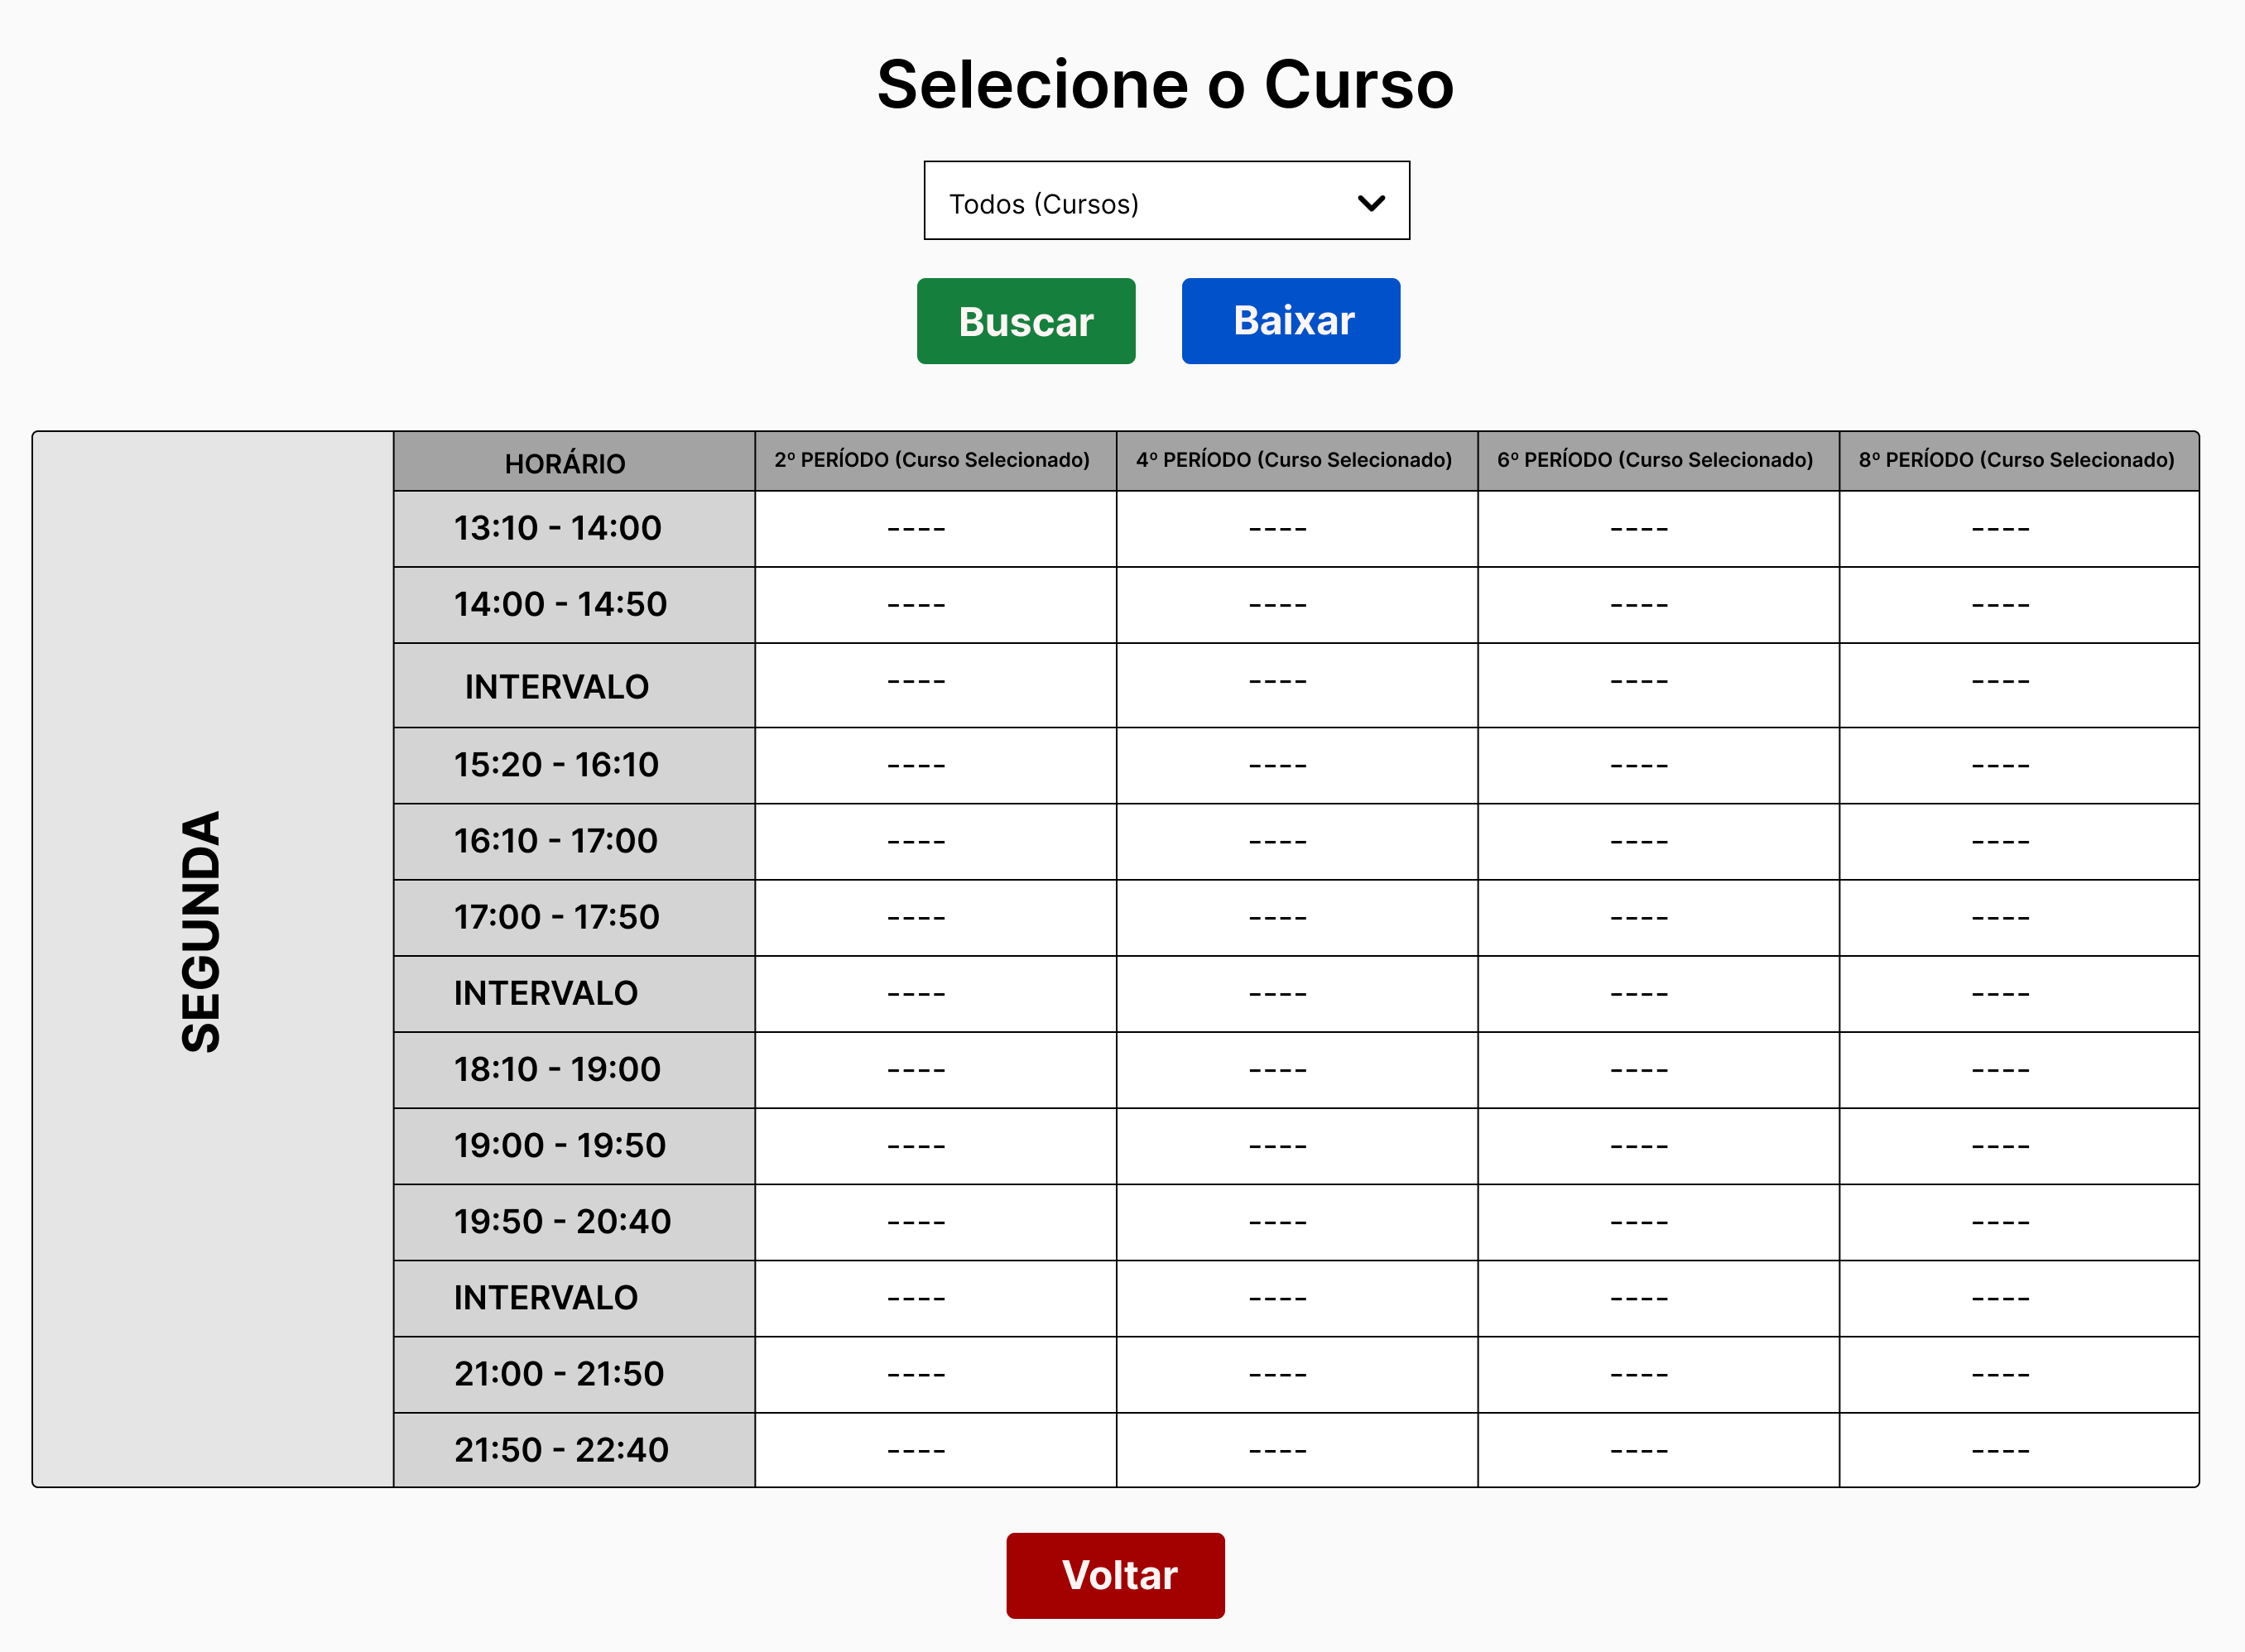
\includegraphics[width=0.7\textwidth]{figuras/proto-3.png}
        \\ % Quebra de linha para separar a imagem da fonte
        \small Fonte: AUTOR (2024)
    \end{figure}
\end{frame}

\begin{frame}{Resultados}
    \begin{figure}
        \centering
        \vspace{-0.5cm}
        \caption{Protótipo da tela dos professores}
        \vspace{-0.2cm}
        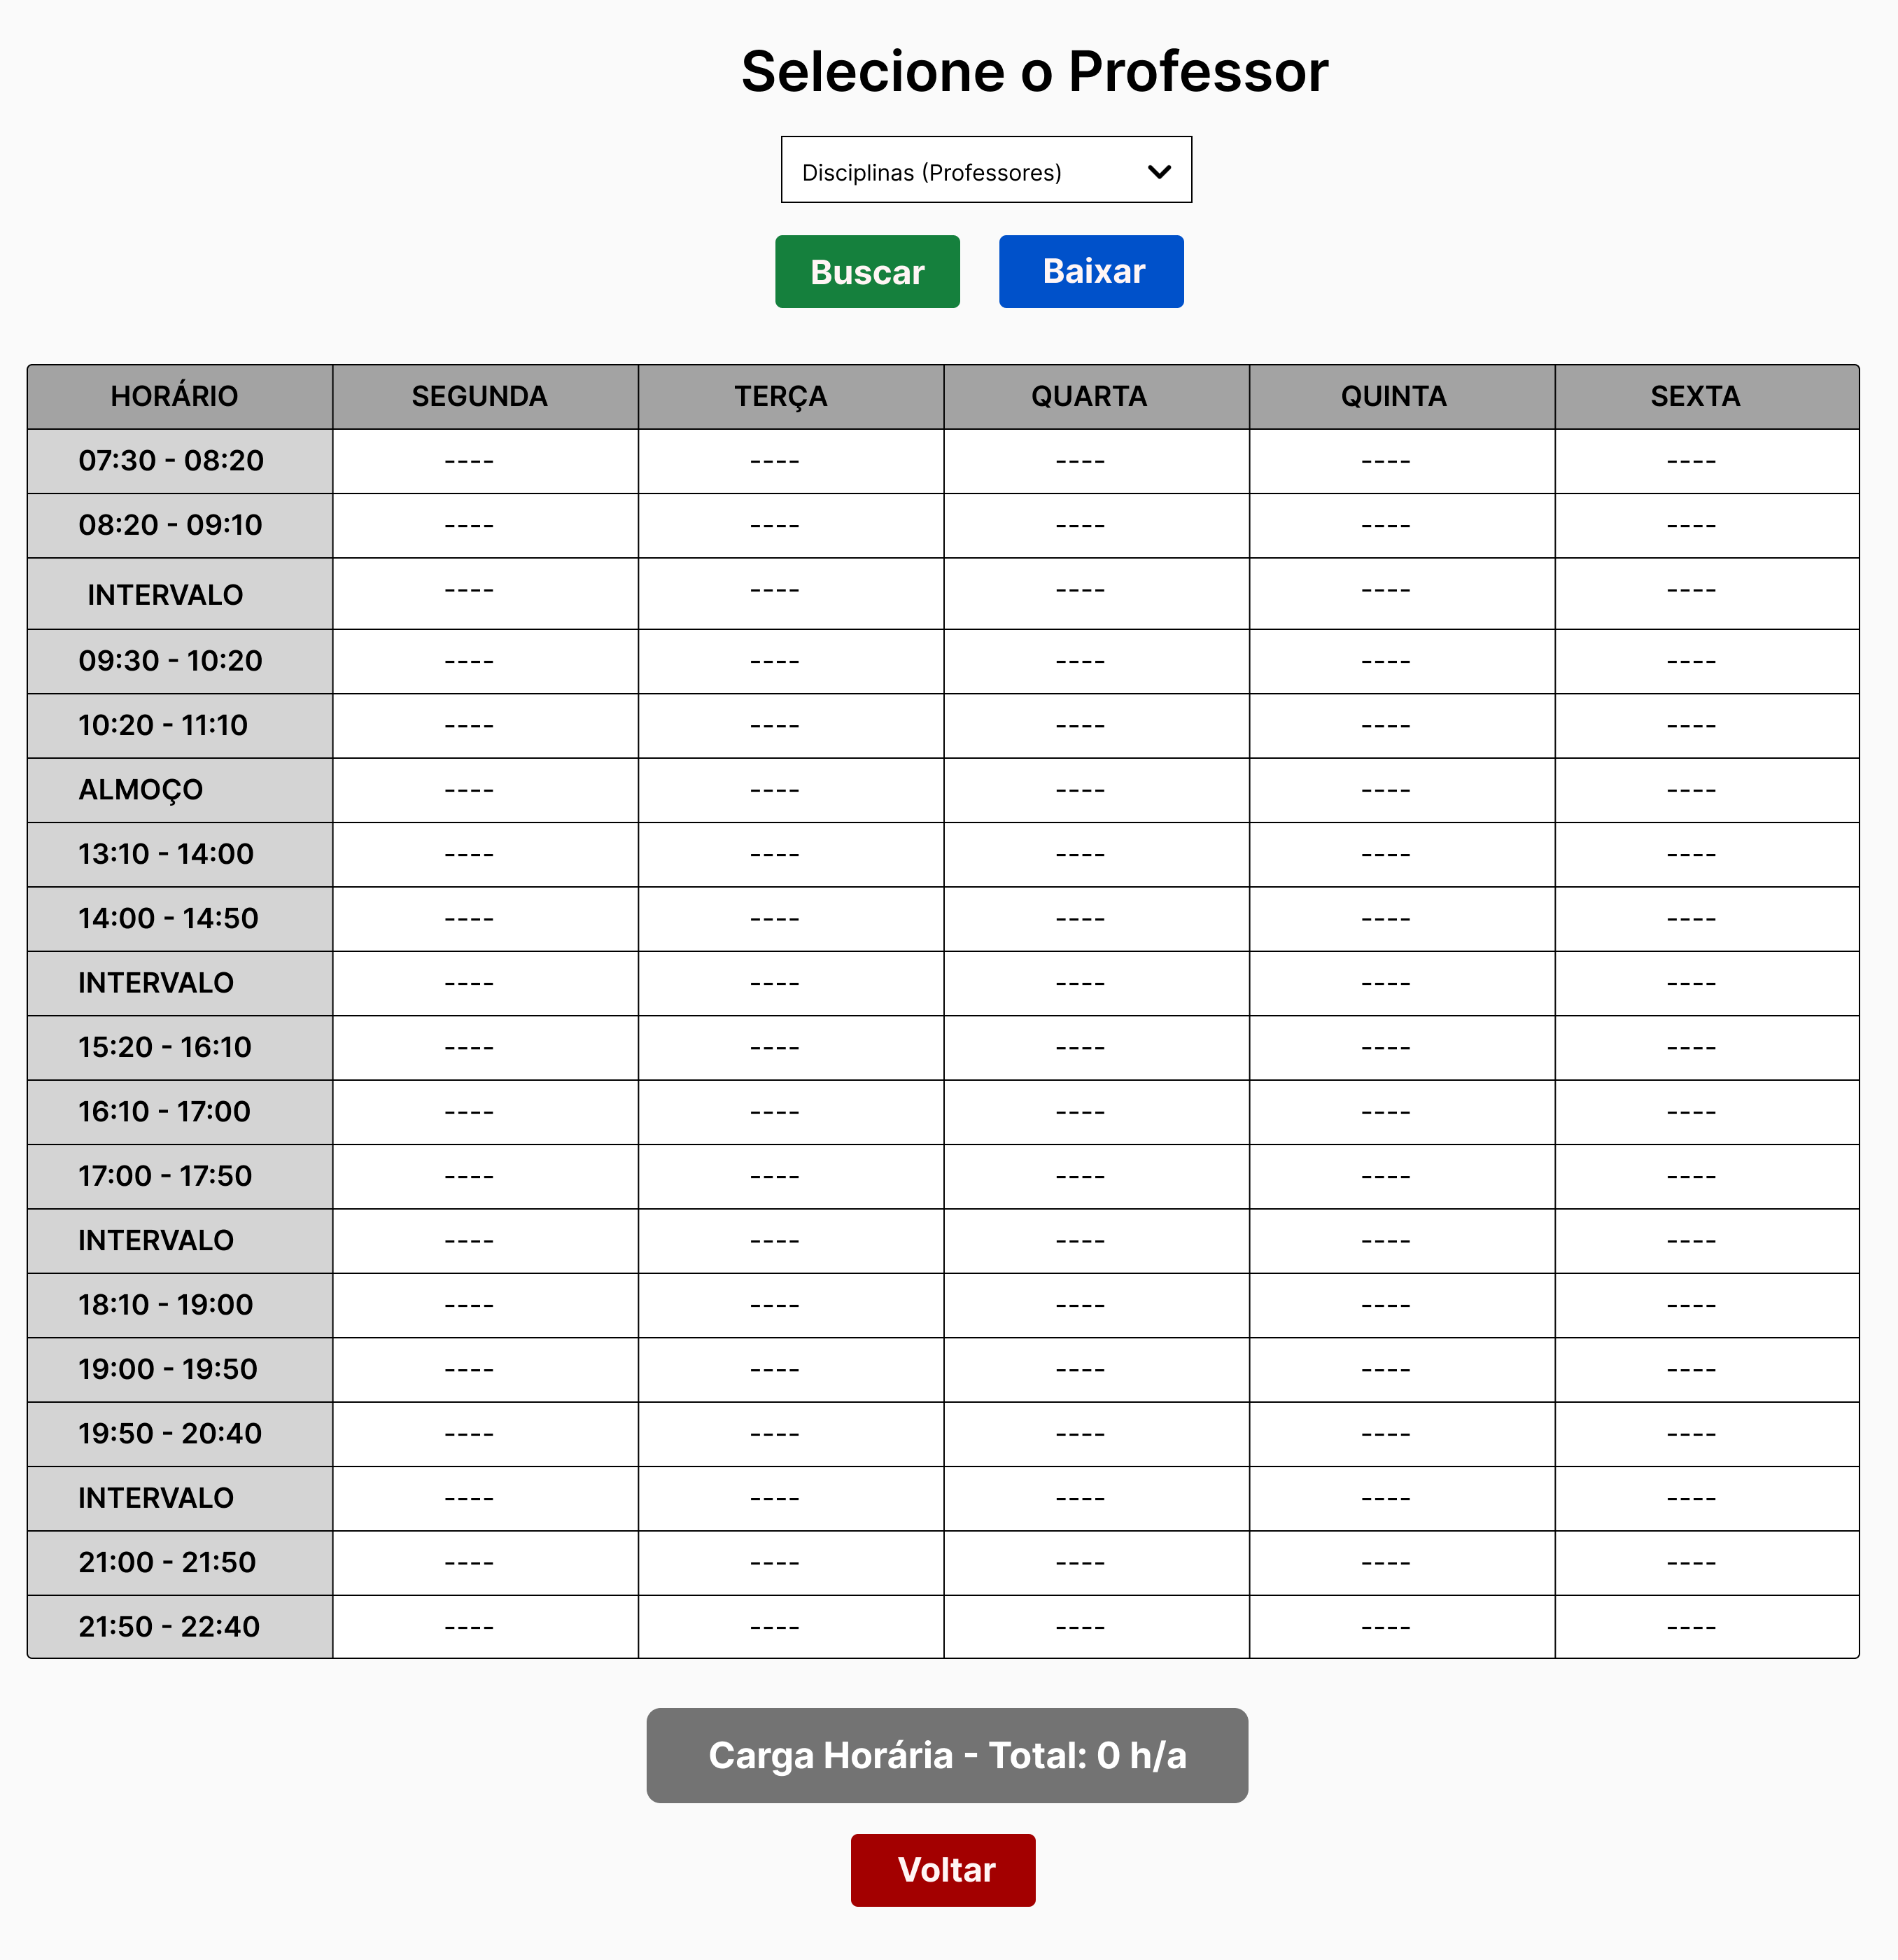
\includegraphics[width=0.5\textwidth]{figuras/proto-4.png}
        \\ % Quebra de linha para separar a imagem da fonte
        \small Fonte: AUTOR (2024)
    \end{figure}
\end{frame}

\begin{frame}{Resultados}
    \begin{figure}
        \centering
        \vspace{-0.5cm}
        \caption{Protótipo da tela das salas}
        \vspace{-0.2cm}
        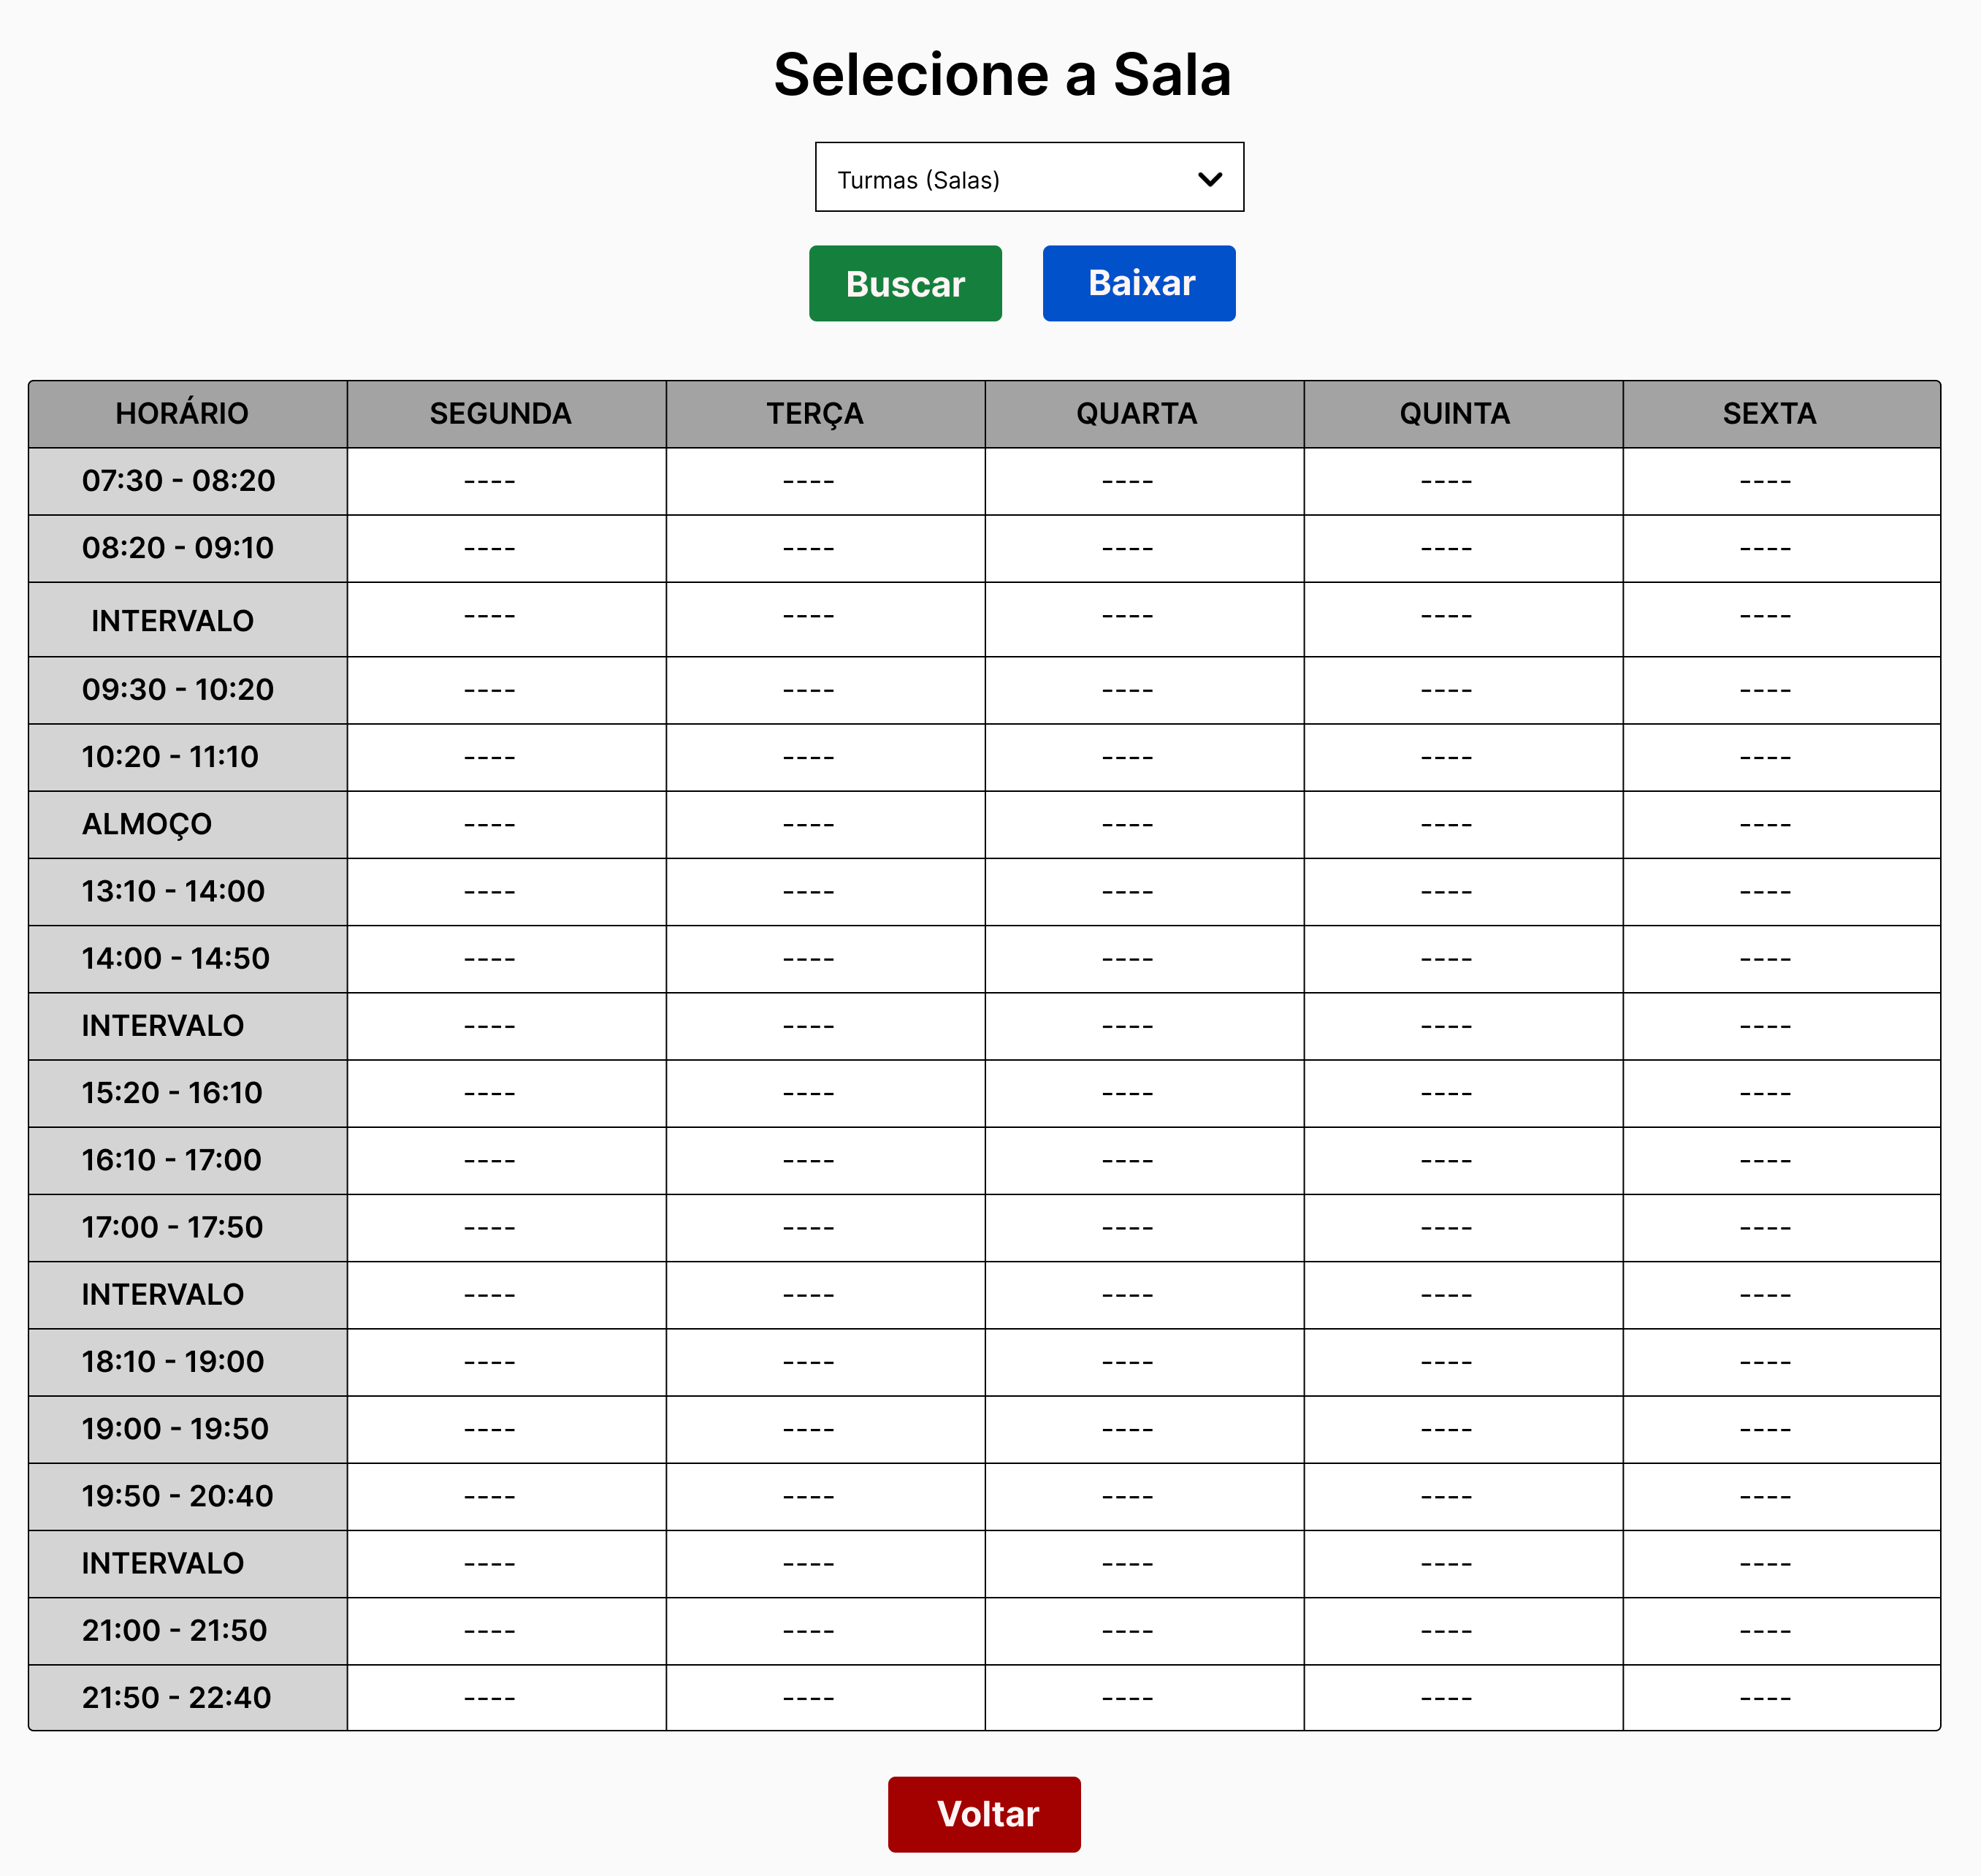
\includegraphics[width=0.5\textwidth]{figuras/proto-5.png}
        \\ % Quebra de linha para separar a imagem da fonte
        \small Fonte: AUTOR (2024)
    \end{figure}
\end{frame}